\documentclass{standalone}
\usepackage{tikz}
\usepackage{tikz-qtree}
\usepackage[makeroom]{cancel}
\usetikzlibrary{fit}


\begin{document} 
	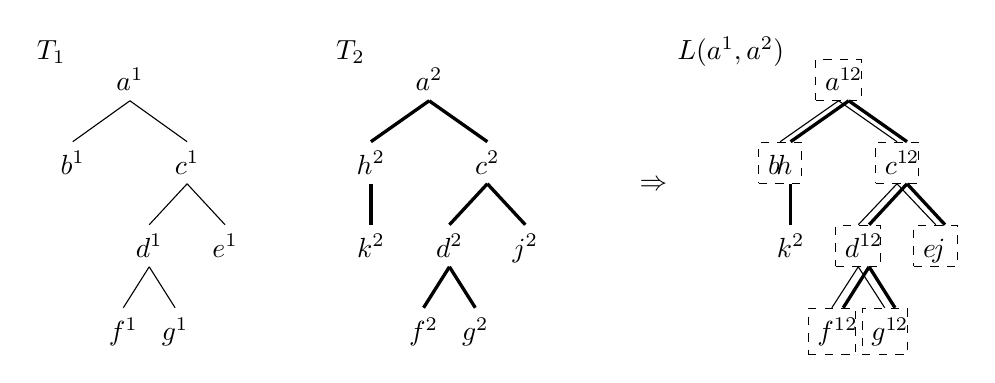
\begin{tikzpicture}[]
	%\tikzset{level 1+/.style={level distance=2.5\baselineskip}}

	    \node (x) at (-1,0.5) {$T_1$};
	    \Tree [.$a^1$
	            [.$b^1$ ] 
	            [.$c^1$ 
	                [.$d^1$ 
	                	[.$f^1$ ]
	                	[.$g^1$ ]
	                ]
	                [.$e^1$ ] 
	            ]
	          ]
	    

	    \begin{scope}[xshift=3.8cm]
	    \tikzset{edge from parent/.style={very thick,draw}}
	    \node (y) at (-1,0.5) {$T_2$} ;
	    \Tree [.$a^2$
	            [.$h^2$ 
	            	[.$k^2$ ]
	            ] 
	            [.$c^2$ 
	                [.$d^2$ 
	                	[.$f^2$ ]
	                	[.$g^2$ ]
	                ]
	                [.$j^2$ ] 
	            ]
	          ]
		\node (arrow1) at (2.85,-1.2) {$\Rightarrow$};
	    \end{scope}



	    \begin{scope}[xshift=9.0cm]
	    %\node (z) at (0,-5.0) {$C_{TO}(a_1^0,a_1^1) = 2$} ;
	    %\tikzset{every tree node/.style={draw=none}}
	    \Tree [.\node[draw,dashed]{$a^1$};
	            [.\node[draw,dashed]{$b\phantom{^1}$}; ] 
	            [.\node[draw,dashed]{$c^1$}; 
	                [.\node[draw,dashed]{$d^1$}; 
	                	[.\node[draw,dashed]{$f^1$}; ]
	                	[.\node[draw,dashed]{$g^1$}; ]
	                ]
	                [.\node[draw,dashed]{$e\phantom{^1}$}; ] 
	            ]
	          ]
	    %\node[draw,dashed,fit=(a)(b)(c)]{};
	    %\node[draw,dashed,fit=(b)(d)(e)]{};
	    \end{scope}



		\begin{scope}[xshift=9.13cm]
		\node (x) at (-1.5,0.5) {$L(a^1,a^2)$};
		\tikzset{edge from parent/.style={very thick,draw}}
	    \Tree [.$\phantom{a}^2$
	            [.$h\phantom{^2}$ 
	            	[.$k^2$ ]
	            ] 
	            [.$\phantom{c}^2$ 
	                [.$\phantom{d}^2$ 
	                	[.$\phantom{f}^2$ ]
	                	[.$\phantom{g}^2$ ]
	                ]
	                [.$j\phantom{^2}$ ] 
	            ]
	          ]
		\end{scope}


	\end{tikzpicture}
\end{document} 